\documentclass[UTF8]{ctexart}
\usepackage{amsmath}
\usepackage{amssymb}
\usepackage{cite}
\usepackage{enumerate}
\usepackage{graphicx}
\usepackage{float}
\usepackage{indentfirst}%设置缩进
\usepackage{booktabs}
\usepackage[numbers,sort&compress]{natbib}
\usepackage[framemethod=TikZ]{mdframed}
\usepackage{url}   % 网页链接
\usepackage{subcaption} % 子标题
\usepackage{listings}


\usepackage{textcomp}
\graphicspath{ {./images/} }
\renewcommand\thesubsubsection{(\arabic{subsubsection})}
%\BeforeBeginEnvironment{tabular}{\zihao{-5}}
\title{\textbf{\kaishu\Huge 第一次数学建模作业}}

\begin{document}
	\maketitle
    \centerline{\Large 第21组成员信息}
        \begin{center}
        \begin{tabular}{ccc}
            \toprule
            姓名 & 班级& 学号\\
            \midrule
            刘沁宇 & 计算机002 &2203613019\\
            徐中伟 & 计算机003 &2206515211 \\
            廉景涛 & 物联网001 &2206113814\\
            \bottomrule
        \end{tabular}
        \end{center}
        \newpage 
    

    \section{火箭分级问题}
        \subsection{问题}
        火箭是一种运输工具,它的任务是将具有一定质量的航天器送入太空。航天器在太空中的运行情况与它进入太空时的初始速度的大小和方向有关。一般地说,如果航天器进入飞行轨道的速度小于第一宇宙速度(7.91千米/秒),航天器将落回地面;
        如果航天器进入轨道的速度介于第一宇宙速度与第二宇宙速度(11.2千米/秒)之间时,它在地球引力场内飞行,成为人造地球卫星;当航天器进入轨道的速度介于第二宇宙速度与第三宇宙速度(16.7千米/秒)之间时,它就飞离地球成为太阳系内
        的人造行星;当航天器进入轨道的速度达到或超过第三宇宙速度时,它就能飞离太阳系。随着人类逐渐进入深空探测和空间飞行器的功能增多,要求火箭具有更大的运载能力,因而出现了多级火箭。多级火箭就是把几个单级火箭连接在一起形成的,
        其中的一个火箭先工作,工作完毕后与其他的火箭分离,然后第二个火箭接着工作,依此类推。由几个火箭组成的就称为几级火箭,如二级火箭、三级火箭,等等。多级火箭的优点是每过一段时间就把不再有用的结构抛弃掉,无需再消耗推进剂来
        带着它和有效载荷(航天器)一起飞行。因此,只要在增加推进剂质量的同时适当地将火箭分成若干级,最终可以使火箭达到足够大的运载能力。然而,级数太多不仅费用增加,可靠性降低,火箭性能也会因结构质量增加而变坏。请建立数学模型,
        分析说明发射卫星为什么一般使用三级火箭系统?
        
        
        \subsection{火箭的升空速度}
        火箭的升空模型本质是物体做反冲运动,火箭携带的燃料燃烧释放大量高速蒸汽,给火箭一个向前的推力。为了便于分析,假设:
        \begin{enumerate}[(i)]
            \item 火箭在上升过程中做直线运动,且不考虑火箭的重力和空气阻力。
            \item 火箭末端喷出的气体相对于火箭的速率$u$为常数。
        \end{enumerate}
        \par 上升模型:设$t$时刻火箭的速率为$v(t)$,火箭的质量为$m(t)$,在$(t,t+\varDelta t)$时间内气体的减少量为$m(t+\varDelta t)-m(t)$,由动量守恒得:
        \begin{equation}
            m(t+\Delta t)v(t+\Delta t) =m(t)v(t)-\left [ m(t+\Delta t)-m(t) \right ]\left [  u-v(t)\right ]
        \end{equation}
        \par 整理可得火箭推进的数学模型为:
        \begin{equation}
            m(t)\frac{\mathrm{d} v(t)}{\mathrm{d} t}=-u\frac{\mathrm{d} m(t)}{\mathrm{d} t}  
        \end{equation}
        \par 令$t=0$,$v(0)=v_0,m(0)=m_0$,解得火箭上升的速度模型为:
        \begin{equation}
            v(t)=v_0+u\ln\frac{m_0}{m(t)} 
        \end{equation}
        \par 因此可得,要想提高火箭的速度,就需要从燃料上增大$u$并从结构上减小$m(t)$。
        
        
        \subsection{一级火箭升空模型}
        \par 设火箭的结构质量为$M_s$(如火箭外壳等),燃料质量为$M_f$,有效负载质量为$M_p$(如卫星等)。查阅资料可得当前$u_{max}=4.2km/s$,且$\frac{M_f}{M_s+M_f+M_p} \le 0.8$。
        \par 对于一级火箭,假设初速度$v_0$忽略不计,
             即$v_0 = 0$ ,且火箭初始质量$m_0=M_f+M_s+M_p$,火箭升空后(燃料耗尽)最终质量为$m_0-M_f$,由公式(3)可得最终速度为
             \begin{equation}
                v=u\ln\frac{m_0}{m_0-M_f}
             \end{equation}
        \par 取$u_{max}=4.2km/s$,$\frac{M_f}{m_0} = 0.8$可得最终速度上限为
        \begin{equation*}
            v_{max}=4.2\times \ln5 \approx 6.76km/s
        \end{equation*}
        \par $v_{max} \le 7.6km/s$因此,用一级火箭发射卫星,在目前技术条件下无法达到相应高度所需的速度。


        \subsection{多级火箭升空模型}
        从一级火箭升空模型可看出火箭推进力自始至终在加速着整个火箭,然而随着燃料的不断消耗,所出现的无用结构质量也在随之不断加速,作了无用功,故效
        益低,浪费大,而而多级火箭可以很好地解决这个问题。多级火箭是从末级开始,逐级燃烧,当第$i$级燃料烧尽时,第$i+1$级火箭立即自动点火,并抛弃已经无用的第$i$级。我们用$m_i$表示第$i$级火箭质量,$M_p$表示有效负载。为了便于分析,作出如下假设:
        \begin{enumerate}[(i)]
            \item 设各级火箭具有相同的$\alpha$,$\alpha m_i$表示第$i$级结构质量,$(1-\alpha)m_i$表示第$i$级的燃料质量。
            \item 喷气相对火箭的速度$u$相同,且第$i$级火箭初始质量与其负载质量之比保持不变,即为$k =\frac{m_i}{m_{i+1}+\cdots m_n+M_p}$($n$为火箭总级数)。
        \end{enumerate}
        \par 对于二级火箭,由(3)式可得,当第一级火箭燃烧完时,火箭此时速度为
        \begin{equation}
            v_1=u\ln \frac{m_1+m_2+M_p}{\alpha m_1+m_2+M_p}=u \ln \frac{k +1}{\alpha k+1} 
        \end{equation}
        \par 在第二级火箭燃烧完时,其速度为
        \begin{equation}
            v_2=v_1+u\ln \frac{m_2+M_p}{\alpha m_2+M_p}=2u \ln \frac{k +1}{\alpha k+1} 
        \end{equation}
        \par 取$u=4.2km/s$,$\alpha=0.2$,考虑空气阻力的影响,为使火箭达到第一宇宙速度$7.6km/s$,$v_2$应比$7.6km/s$大,这里取$v_2=10km/s$ .由公式(6)可得
        \begin{equation*}
            10=2\times4.2\times\ln \frac{k+1}{0.2k+1} 
        \end{equation*}
        \par 解得
        \begin{equation*}
            k\approx 6.69
        \end{equation*}
        \par 此时
        \begin{equation*}
            \frac{m_0}{M_p}=\frac{m_1+m_2+M_p}{M_p}= (k+1)^2\approx 60  
        \end{equation*}
        \par 同理,可推出三级火箭
        \begin{equation*}
            v_{3}=3 u \ln \frac{k+1}{\alpha k+1}
        \end{equation*}
        \par 欲使$v_3 = 10.5 km/s$,应该$k\approx 2.17$,从而$\frac{m_0}{M_p}=(k+1)^3\approx 32$。
        \par 与二级火箭相比,在达到相同效果的情况下,三级火箭的质量几乎节省了一半。
        \par 现记$n$级火箭的总质量(包括有效负载$M_p$)为$m_0$,在相同假设下($u = 3 km/s,v_末= 10km/s,\alpha= 0.2$),可以算出相应的$\frac{m_0}{M_p}$值,现将计算结果列于下表中:
        \begin{center}
            \begin{tabular}{ccccccccc}
                \toprule
                    $n$ (级数)&1 & 2 &  3 & 4 &   5 & 6 & $\cdots$ & $\infty$ \\
                    $\frac{m_0}{M_p}$& $\oslash $& 60 & 32 & 27&  24 & 23& $\cdots$ & 19 \\
                \bottomrule
            \end{tabular}
            \end{center}
       
    \subsection{结论}
    在火箭发射的问题中,一级火箭无法完成发射任务,在多级火箭中,三级火箭更符合经济效益,且技术限制相对较小。
    \newpage

    \section{卫星测控问题}
    \setcounter{equation}{0}
        设$R$为地球半径,$h$为运行轨道距离地球表面的距离,$a$为观测站所能观测到得最大倾角的一半,a=87° 。
        为了便于分析,现做出以下假设:
        \begin{enumerate}[(i)]
            \item 假设地球为标准的球体,且地球自转时为刚体运动。
            \item 假设卫星的环绕运动以地心为中心点的圆,卫星在赤道附近运动,所在平面与赤道夹角很小。
        \end{enumerate}

        \subsection{问题一}
        因为所求为最少数量,所以假设两个条件:
        \begin{enumerate}[(i)]
            \item 卫星运动平面和赤道共平面。
            \item 检测站同样位于赤道。
        \end{enumerate}
        \par 模型简化为:
        \begin{figure}[!htbp]
            \centering
            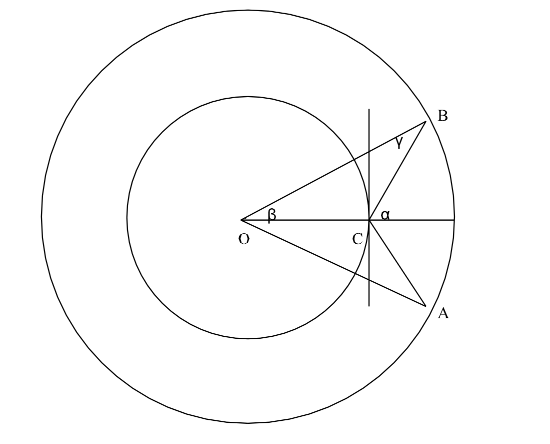
\includegraphics[width=0.45\textwidth]{第一问}
            \caption{测控站与卫星共面模型} 
        \end{figure}
        \par 由几何关系可得:
        \begin{align}
            OB =OA&=R+h\\
            \frac{\sin (a-\beta)}{R} &=\frac{\sin (\pi-a)}{R+h}\\
        \end{align}
        \par 可解得$\beta$的值为:
        \begin{equation}
            \beta =a-\arcsin (\frac{R \sin a}{R+h})
        \end{equation}
        \par 由于监测站检测的位置要覆盖整个卫星的运行轨道,故有$2\pi <2n \beta$,所以至少要设立的就监测站数量为:
        \begin{equation}
            n=[\frac{\pi}{\beta}]+1
        \end{equation}

        \subsection{问题二}
        为了简化计算,本题假设卫星所在轨道平面角度不会影响监测站在环形面上的投影形状(为圆)。
        \begin{figure}[H]
            \centering %图片全局居中
            %并排几个图,就要写几个minipage
            \begin{minipage}[b]{0.45\textwidth} %所有minipage宽度之和要小于1,否则会自动变成竖排
            \centering %图片局部居中
            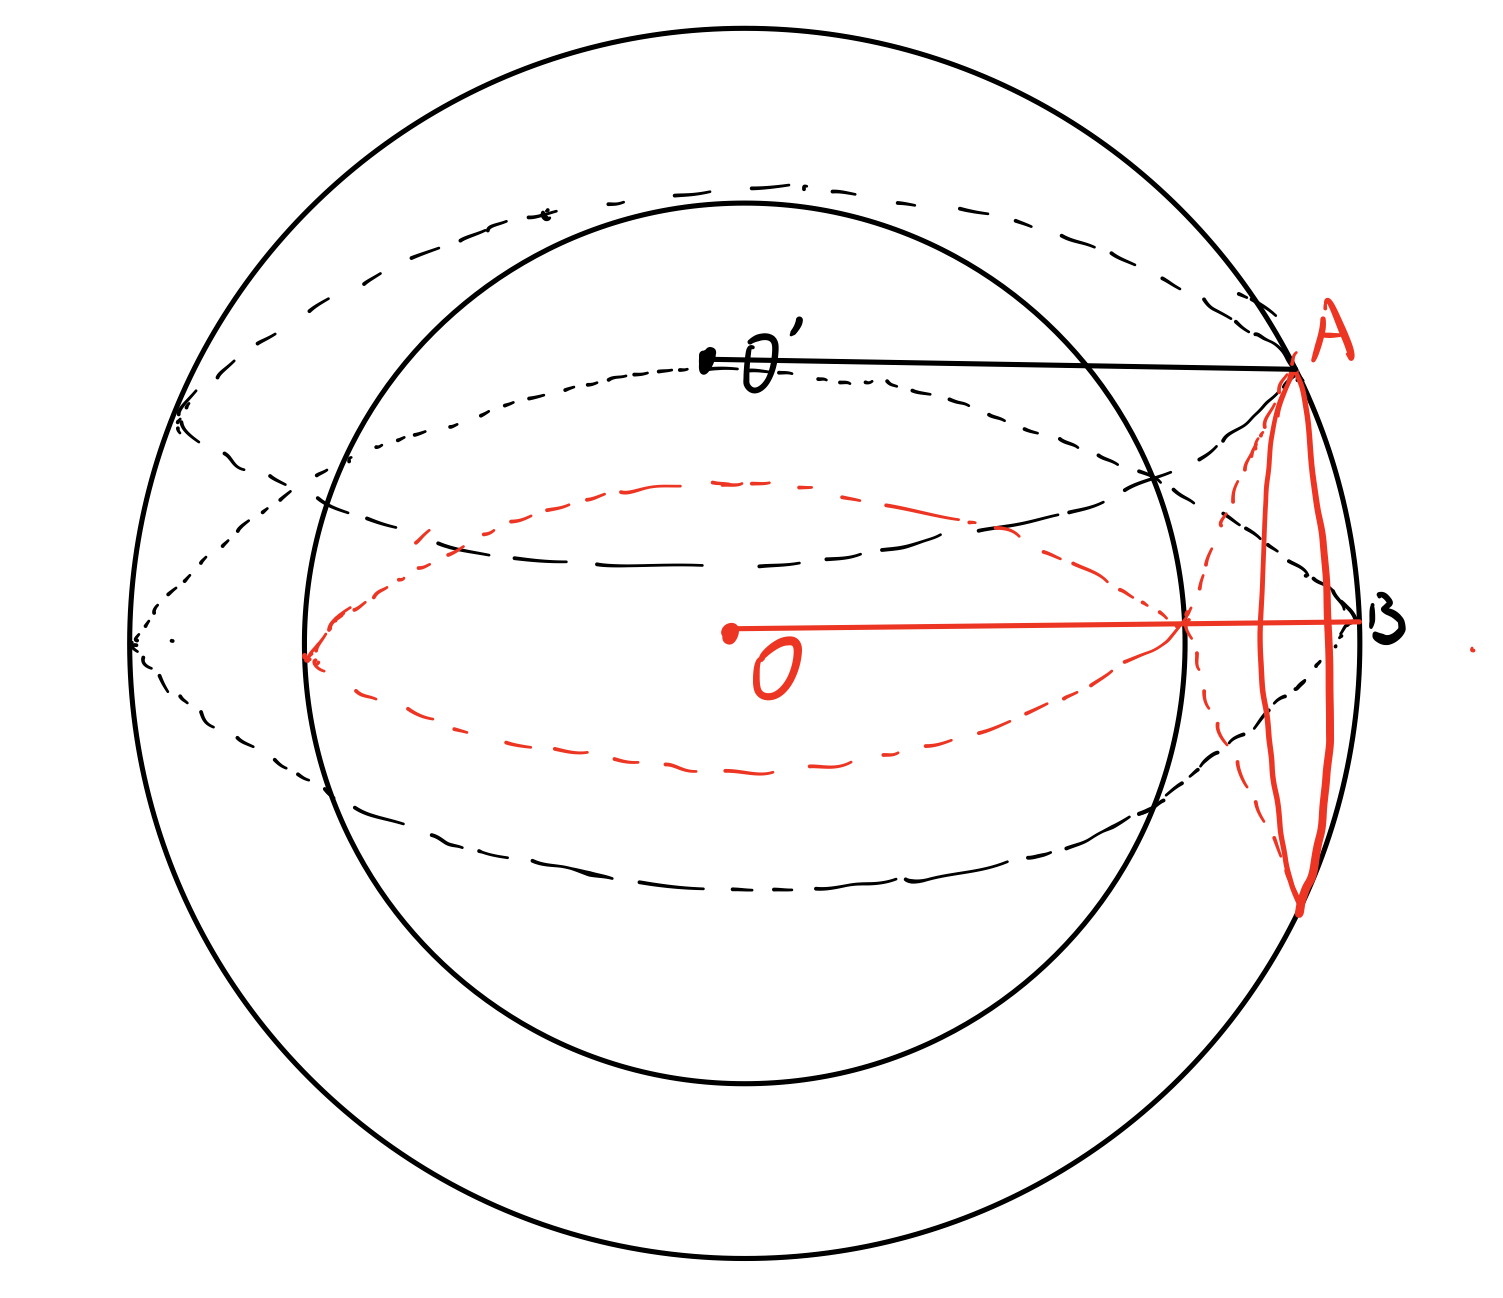
\includegraphics[width=0.8\textwidth]{第二问1} %此时的图片宽度比例是相对于这个minipage的,不是全局
            \caption{空间图}
            \label{Fig.1}
            \end{minipage}
            \begin{minipage}[b]{0.45\textwidth} %所有minipage宽度之和要小于1,否则会自动变成竖排
            \centering %图片局部居中
            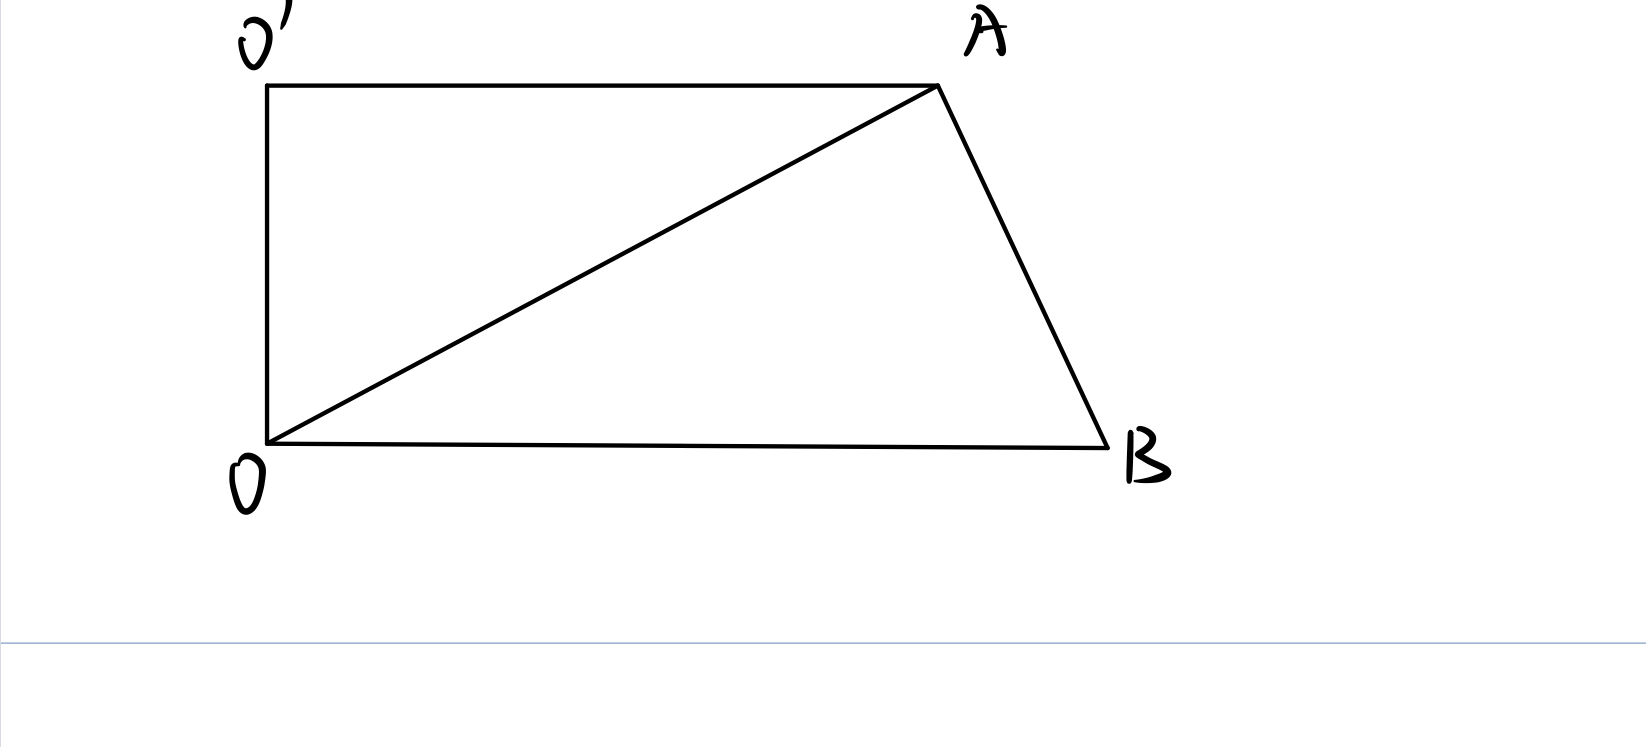
\includegraphics[width=0.8\textwidth]{第二问2}%此时的图片宽度比例是相对于这个minipage的,不是全局
            \caption{剖面图}
            \label{Fig.2}
            \end{minipage}
        \end{figure}
        \par 令$\angle AOB=\angle \beta$,先讨论角M较小情况:由题目条件知,$OA=OB=R+h$, 而角$\beta$为卫星运行轨道与赤道平面之间的夹角时,当运行轨道确定时,$\beta$的值是确定的,因此可以作为已知条件。由几何三角知识可知,满足下列条件:
        \begin{align}
            OA &=(R+h) \cos \beta\\
            OO'&=(R+h) \sin B
        \end{align}
        \par 又有:
        \begin{figure}[!htbp]
            \centering
            \includegraphics*[width=0.45\textwidth]{第二问3}
        \end{figure}
        \begin{align}
            OC&=OE=R+h=OH_1=OH_2\\
            IH_0&=OO'
        \end{align}
        \par 而从第一问中,我们可以根据观测站的最大检测角度$a$求出$\beta $的值,在这里D为监测站的位置,所以$OI=(R+h)\cos \beta$,
             再由勾股定理得:
        \begin{align}
            (OH_0)^2 & =(IH_0)^2+(OB)^2\\
            (H_1H_0)^2 & =(R+h)^2-(OH_0)^2
        \end{align}
        \par 从O'O的方向看便转成题一求法:
        \begin{figure}
            \centering
            \includegraphics*[width=0.45\textwidth]{第二问4}
        \end{figure}
        \par $OH_1=OH_2=OA$,这在(1)中已经求出,现在,我们只需求出角$\theta$,便可以将问题回溯到第一问的模型上。
        \par 由三角形知识可得:
        \begin{equation}
            \beta =\arcsin \frac{H_0H_1}{OH_1} =\arcsin \frac{H_0H_1}{OA}
        \end{equation}
        \par 此时$\beta $是$\angle H_2OA$,大小和前面的不一样。此时所需的监测站至少为:
        \begin{equation*}
            n=[\frac{\pi}{\beta}]+1
        \end{equation*}
        \begin{figure*}[!htbp]
            \centering
            \includegraphics*[width=0.45\textwidth]{第二问5}
            \caption{如果平面角度较大,则会导致$H_0I$过大}
        \end{figure*}
        \newpage
        \par 简化模型有:
        \begin{figure}
            \centering
            \includegraphics*[width=0.45\textwidth]{第二问6}
        \end{figure}
        \begin{align*}
            QS &=R\\
            ST \le &\frac{3}{2} R\\
            (PT)^2 &=R^2-(ST-R)^2
        \end{align*}
        \par 而这里的$PT$就相当于题一中的$H_0H_1$,而$ST$就相当于题一中的$IH_0$;故可以将求解出的$PT$代入题一的公式中进行下一步的求解;
              此时由于检测站的位置发生了变化,故卫星能够达到的相对地心的高度也改变了;但我们事先知道卫星运行轨迹 与赤道之间的夹角,故可以将题一中的算式做相应的调整: 
        \begin{equation}
            IH_1=(R+h)\sin \beta
        \end{equation}
        \par 其中$\beta_0$为已知的轨迹与赤道夹角.又因为此时我们是在赤道的两侧建立检测站, 故至少需要检测站的个数$N' =2N$。
        


















    \newpage
    \section{废水排污问题}
    \setcounter{equation}{0}
    \setcounter{figure}{0}
    \subsection{问题}
    设一个化工厂每立方米的废水中含有$3.08kg$盐酸,这些废水经过一条河流流入一个湖泊中,废水流入的速率为$20m^3/s$。
    开始时湖中有水$4000000m^3$,河流中流入湖泊的不含盐酸的水是$1000m^3/s$,湖泊中混合水的流出速率是$1000m^3/s$。
    求该厂排污开始一年后时,湖泊中盐酸的含量。
	
    \subsection{模型建立}
    设$t$时刻湖泊中含有的盐酸质量为$x(t)(kg)$,考虑$[t,t+\Delta t]$时间内湖泊中盐酸的变化:
    \begin{equation}
        x(t+\Delta t)-x(t)=20 \times 3.08\Delta t + \frac{1000x(t)}{4000000+20t} \Delta t
    \end{equation}
    \par 因此有
    \begin{equation}
        \frac{\mathrm{d} x}{\mathrm{d} t}+\frac{1000x}{4000000+20t}=61.6,\\x(0)=0 
    \end{equation}
    \par 该微分方程的解为
    \begin{equation}
       x(t)=1.20784 \ldots(t+200000)-\frac{200000^{50} \cdot 241568}{(200000+t)^{50}}
    \end{equation}
    \par 一年后,湖泊水中的盐酸含量为
    \begin{equation*}
        x(24\times 365)\approx 223815(kg)
    \end{equation*}

    \subsection{结论}
    解决废水排污问题本质是构建常微分方程模型,再根据0时刻的值求方程的解。

    \newpage
    \section{鲸的种群增长问题}
    \setcounter{equation}{0}
    
    \subsection{问题}
    蓝鲸和长须鲸是两个生活在同一海域的形似的种群,蓝鲸的内禀增长率每年估计为5\%,长须鲸为8\%。
    蓝鲸的环境容纳量为150000条,长须鲸为400000条。目前蓝鲸大约为5000条,长须鲸大约为70000条。如果
    不考虑捕捞,两种鲸鱼种群回到自然水平需要多长时间?
    \subsection{模型建立}
    若只单独考虑某个种群的增长,可应用种群增长的Logistic模型:
    \begin{equation}
        \frac{\mathrm{d} N(t)}{\mathrm{d} t}=r(1-\frac{N(t)}{K})N(t)
    \end{equation}
    \par $N(t)$表示时刻$t$种群数量,$r$表示种群的内禀增长速率,$K$表示环境容纳量。
    \par 对于两个以上的种群,则可以建立种群的竞争模型。用$N_1(t)$和$N_2(t)$分别表示在$t$时刻蓝鲸和长须鲸两个种群的数量,并作出以下假设:
    \begin{enumerate}[(i)]
        \item 当某种群单独存在时,遵循种群变化的的Logistic规律,即\\
        
        \begin{center} $ \frac{\mathrm{d} N_i(t)}{\mathrm{d} t}=r_i(1-\frac{N_i(t)}{K_i})N_i(t)$ \end{center}
        \item 增加一个竞争对手所导致的平均增长率的降低量正比于竞争对手的单位数量($\frac{N_i}{K_i}$)。
    \end{enumerate}  
    \par 设两种鲸鱼之间的竞争力的影响因子为$\alpha _i$,$\alpha _1$的含义是单位数量的长须鲸(相对于$K_2$)消耗的供养蓝鲸的资源量为单位数量蓝鲸(相对于$K_1$)消耗的供养蓝鲸资源量的$\alpha _1$倍:
    \begin{align}
        \frac{\mathrm{d} N_1}{\mathrm{d} t} &=r_1N_1(1-\frac{N_1}{K_1}-\alpha_1 \frac{N_2}{K_2}) \\
        \frac{\mathrm{d} N_2}{\mathrm{d} t} &=r_2N_2(1-\frac{N_2}{K_2}-\alpha_2 \frac{N_1}{K_1})
    \end{align}
    % \par 该微分方程组的矩阵形式是
    % \begin{equation}
    %     \frac{\mathrm{d} }{\mathrm{d} x} \begin{bmatrix} N_1\\N_2 \end{bmatrix}=
    % \begin{bmatrix}
    %     -\frac{r_1}{K_1}  &  -\alpha \\
    %     -\frac{r_2}{K_2}  &  -\alpha 
    %     \end{bmatrix}
    %     \begin{bmatrix}
    %     N_1\\N_2
    %     \end{bmatrix}
    %     +
    %     \begin{bmatrix}
    %     r_1\\r_2
    %     \end{bmatrix}
    % \end{equation}
    \par 为了便于分析,假设两种生物之间的竞争力是相同的,即$\alpha _1=\alpha_2$。由于蓝鲸和长须鲸的生活习性相近,因此考虑$\alpha$的值在$[0.1,1]$范围内,这里对该范围内的$\alpha$取不同的值进行拟合,得到以下实验结果:
    \newpage

    \begin{figure}[H]
        \centering
        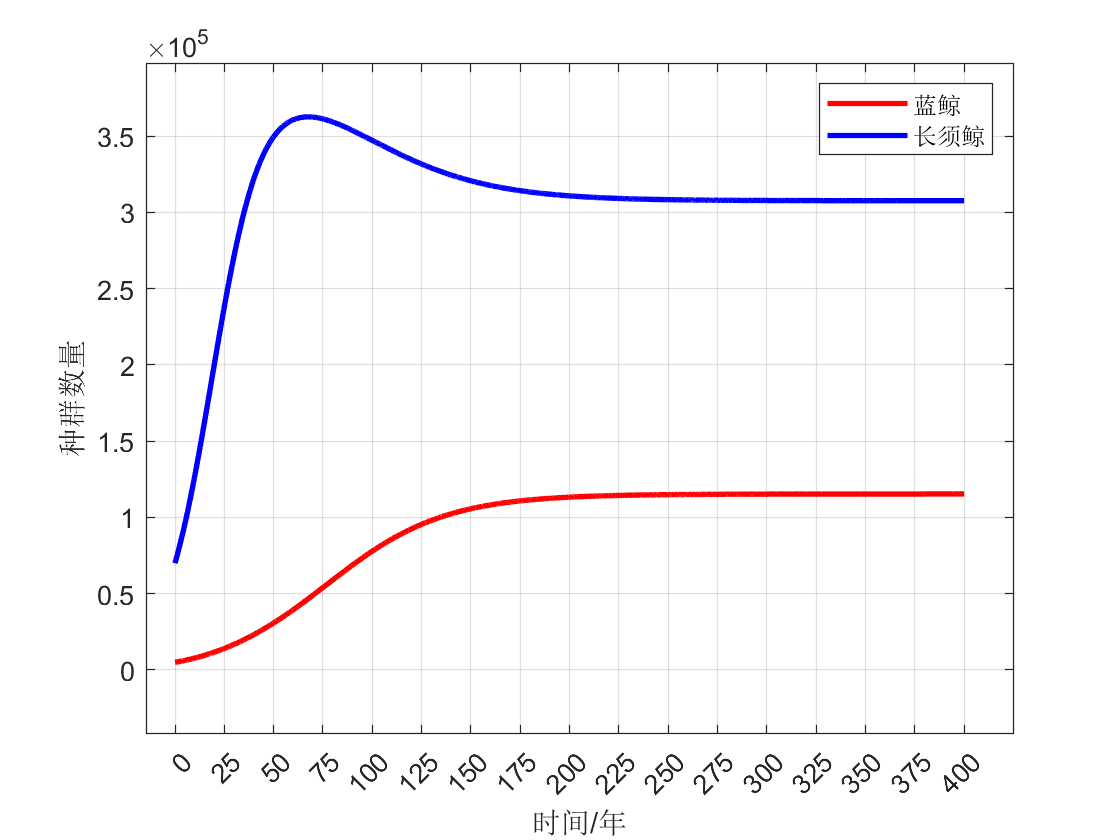
\includegraphics[scale=0.3]{a=0.3}
        \caption{$\alpha=0.3$}
        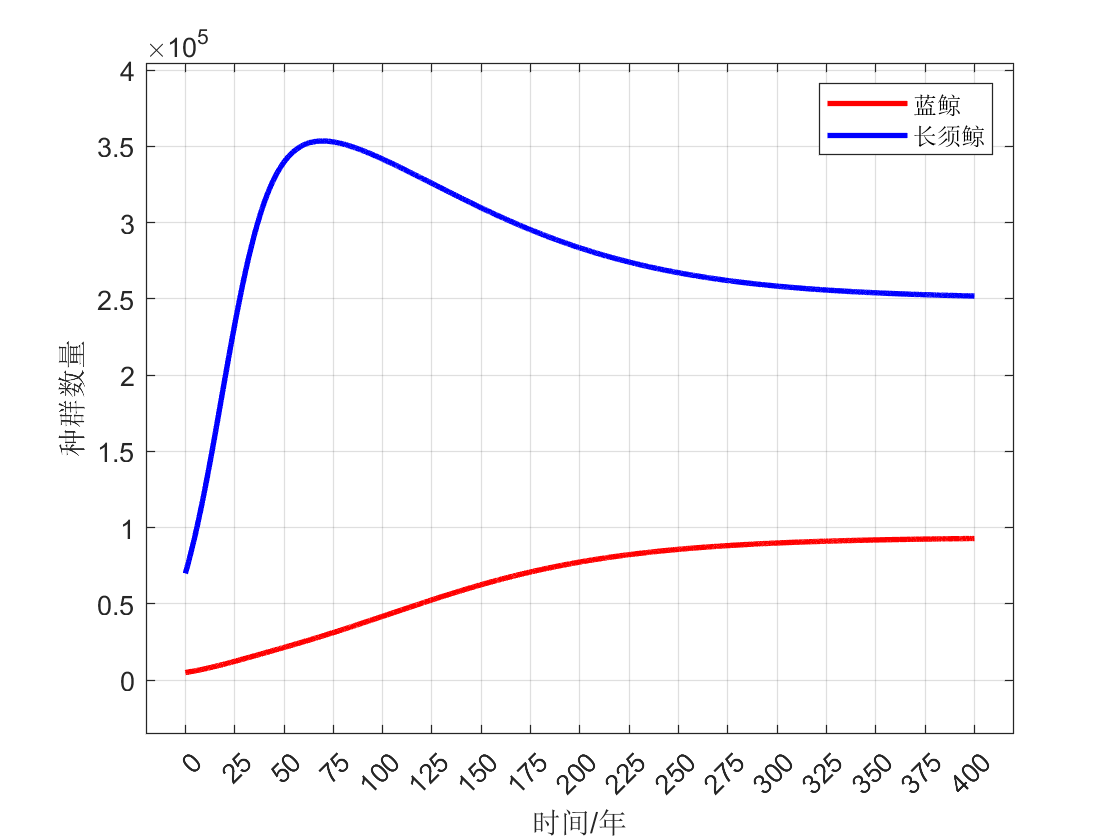
\includegraphics[scale=0.3]{a=0.6}
        \caption{$\alpha=0.6$}
        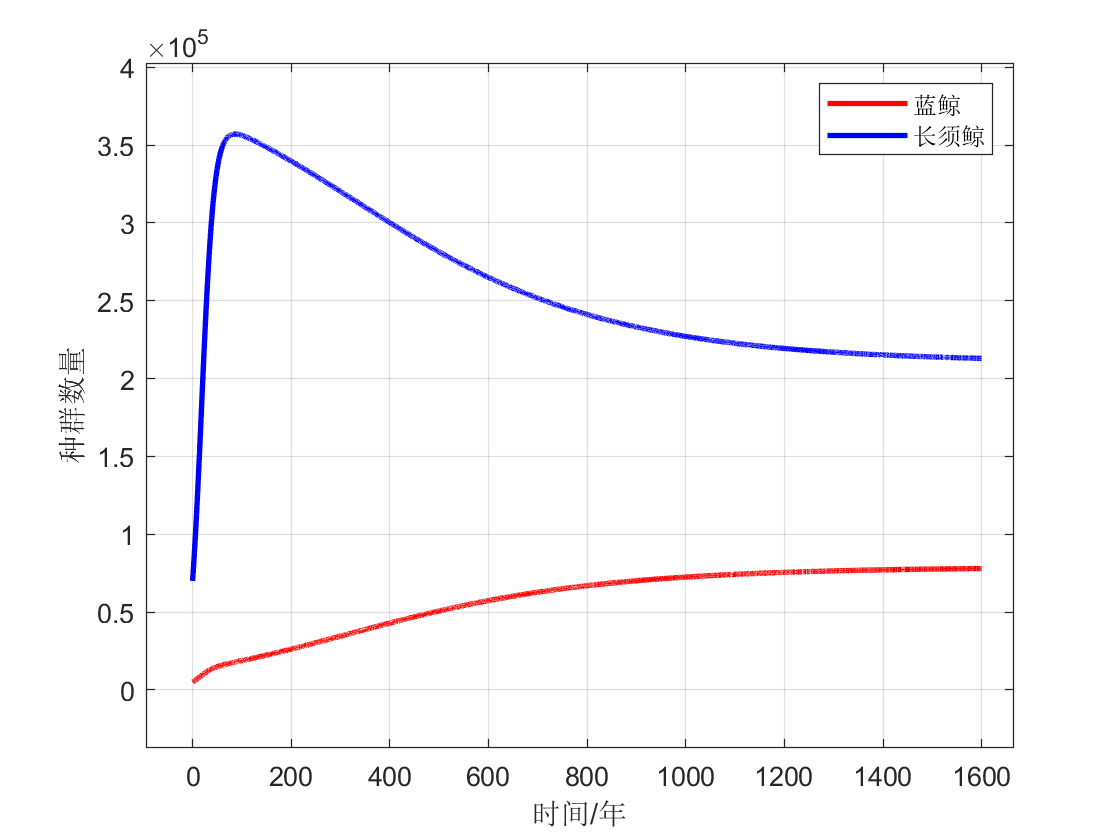
\includegraphics[scale=0.3]{a=0.9}
        \caption{$\alpha=0.9$}
    \end{figure}
    
    \subsection{结论}
    不同$\alpha$下的两种鲸的回归自然水平所需时间以及最终种群数量如下表:
    \begin{table}[!htbp]
        \centering
           
                \begin{tabular}{cccc}
                    \toprule
            $\alpha$ & 0.3& 0.6& 0.9\\
                    \midrule
            所需时间/年 & 200 & 325 & 1200\\
            最终数量/($\times 10^5$) & 1.2 & 0.9 & 0.7\\
                    \bottomrule
                    
                \end{tabular}
                \caption{蓝鲸种群变化}
               
            
            
                \begin{tabular}{cccc}
                    \toprule
            $\alpha$ & 0.3& 0.6& 0.9\\
                    \midrule
            所需时间/年 & 225 & 400 & 1600\\
            最终数量/($\times 10^5$) & 3.1 & 2.5 & 2.2\\
                    \bottomrule
                \end{tabular}
                \caption{长须鲸种群变化}
    \end{table}  

    \subsection{代码附录}
    
    \begin{lstlisting}	%正文插入代码
        function dx=fun(t,x,r1,r2,n1,n2,s1,s2)
        r1=0.05;
        r2=0.08;
        n1=150000;
        n2=400000;
        s1=0.9;
        s2=0.9;
        dx=[r1*x(1)*(1-x(1)/n1-s1*x(2)/n2);r2*x(2)*(1-s2*x(1)/n1-x(2)/n2)];
        \%main.m
        clc;
        clear;
        h=0.1;
        ts=[0:h:1600];
        x0=[5000,70000];
        opt=odeset('reltol',1e-6,'abstol',1e-9);
        [t,x]=ode45(@fun,ts,x0,opt);
        xlabel('-2\pi < x < 2\pi') ;
        ylabel('Sine and Cosine Values');
        plot(t,x(:,1),'r',t,x(:,2),'b','LineWidth',2),grid;
    \end{lstlisting}

\end{document}